\documentclass[twoside]{book}

% Packages required by doxygen
\usepackage{fixltx2e}
\usepackage{calc}
\usepackage{doxygen}
\usepackage[export]{adjustbox} % also loads graphicx
\usepackage{graphicx}
\usepackage[utf8]{inputenc}
\usepackage{makeidx}
\usepackage{multicol}
\usepackage{multirow}
\PassOptionsToPackage{warn}{textcomp}
\usepackage{textcomp}
\usepackage[nointegrals]{wasysym}
\usepackage[table]{xcolor}

% Font selection
\usepackage[T1]{fontenc}
\usepackage[scaled=.90]{helvet}
\usepackage{courier}
\usepackage{amssymb}
\usepackage{sectsty}
\renewcommand{\familydefault}{\sfdefault}
\allsectionsfont{%
  \fontseries{bc}\selectfont%
  \color{darkgray}%
}
\renewcommand{\DoxyLabelFont}{%
  \fontseries{bc}\selectfont%
  \color{darkgray}%
}
\newcommand{\+}{\discretionary{\mbox{\scriptsize$\hookleftarrow$}}{}{}}

% Page & text layout
\usepackage{geometry}
\geometry{%
  a4paper,%
  top=2.5cm,%
  bottom=2.5cm,%
  left=2.5cm,%
  right=2.5cm%
}
\tolerance=750
\hfuzz=15pt
\hbadness=750
\setlength{\emergencystretch}{15pt}
\setlength{\parindent}{0cm}
\setlength{\parskip}{3ex plus 2ex minus 2ex}
\makeatletter
\renewcommand{\paragraph}{%
  \@startsection{paragraph}{4}{0ex}{-1.0ex}{1.0ex}{%
    \normalfont\normalsize\bfseries\SS@parafont%
  }%
}
\renewcommand{\subparagraph}{%
  \@startsection{subparagraph}{5}{0ex}{-1.0ex}{1.0ex}{%
    \normalfont\normalsize\bfseries\SS@subparafont%
  }%
}
\makeatother

% Headers & footers
\usepackage{fancyhdr}
\pagestyle{fancyplain}
\fancyhead[LE]{\fancyplain{}{\bfseries\thepage}}
\fancyhead[CE]{\fancyplain{}{}}
\fancyhead[RE]{\fancyplain{}{\bfseries\leftmark}}
\fancyhead[LO]{\fancyplain{}{\bfseries\rightmark}}
\fancyhead[CO]{\fancyplain{}{}}
\fancyhead[RO]{\fancyplain{}{\bfseries\thepage}}
\fancyfoot[LE]{\fancyplain{}{}}
\fancyfoot[CE]{\fancyplain{}{}}
\fancyfoot[RE]{\fancyplain{}{\bfseries\scriptsize Generated by Doxygen }}
\fancyfoot[LO]{\fancyplain{}{\bfseries\scriptsize Generated by Doxygen }}
\fancyfoot[CO]{\fancyplain{}{}}
\fancyfoot[RO]{\fancyplain{}{}}
\renewcommand{\footrulewidth}{0.4pt}
\renewcommand{\chaptermark}[1]{%
  \markboth{#1}{}%
}
\renewcommand{\sectionmark}[1]{%
  \markright{\thesection\ #1}%
}

% Indices & bibliography
\usepackage{natbib}
\usepackage[titles]{tocloft}
\setcounter{tocdepth}{3}
\setcounter{secnumdepth}{5}
\makeindex

% Hyperlinks (required, but should be loaded last)
\usepackage{ifpdf}
\ifpdf
  \usepackage[pdftex,pagebackref=true]{hyperref}
\else
  \usepackage[ps2pdf,pagebackref=true]{hyperref}
\fi
\hypersetup{%
  colorlinks=true,%
  linkcolor=blue,%
  citecolor=blue,%
  unicode%
}

% Custom commands
\newcommand{\clearemptydoublepage}{%
  \newpage{\pagestyle{empty}\cleardoublepage}%
}

\usepackage{caption}
\captionsetup{labelsep=space,justification=centering,font={bf},singlelinecheck=off,skip=4pt,position=top}

%===== C O N T E N T S =====

\begin{document}

% Titlepage & ToC
\hypersetup{pageanchor=false,
             bookmarksnumbered=true,
             pdfencoding=unicode
            }
\pagenumbering{alph}
\begin{titlepage}
\vspace*{7cm}
\begin{center}%
{\Large My Project }\\
\vspace*{1cm}
{\large Generated by Doxygen 1.8.14}\\
\end{center}
\end{titlepage}
\clearemptydoublepage
\pagenumbering{roman}
\tableofcontents
\clearemptydoublepage
\pagenumbering{arabic}
\hypersetup{pageanchor=true}

%--- Begin generated contents ---
\chapter{Namespace Index}
\section{Namespace List}
Here is a list of all documented namespaces with brief descriptions\+:\begin{DoxyCompactList}
\item\contentsline{section}{\mbox{\hyperlink{namespace_ui}{Ui}} }{\pageref{namespace_ui}}{}
\end{DoxyCompactList}

\chapter{Hierarchical Index}
\section{Class Hierarchy}
This inheritance list is sorted roughly, but not completely, alphabetically\+:\begin{DoxyCompactList}
\item \contentsline{section}{Creator}{\pageref{class_creator}}{}
\begin{DoxyCompactList}
\item \contentsline{section}{Simple\+Creator}{\pageref{class_simple_creator}}{}
\end{DoxyCompactList}
\item \contentsline{section}{Graphic}{\pageref{class_graphic}}{}
\begin{DoxyCompactList}
\item \contentsline{section}{Ball}{\pageref{class_ball}}{}
\begin{DoxyCompactList}
\item \contentsline{section}{Composite\+Ball}{\pageref{class_composite_ball}}{}
\item \contentsline{section}{Simple\+Ball}{\pageref{class_simple_ball}}{}
\end{DoxyCompactList}
\item \contentsline{section}{Scene\+Manager}{\pageref{class_scene_manager}}{}
\item \contentsline{section}{Table}{\pageref{class_table}}{}
\begin{DoxyCompactList}
\item \contentsline{section}{Pocket\+Table}{\pageref{class_pocket_table}}{}
\item \contentsline{section}{Simple\+Table}{\pageref{class_simple_table}}{}
\end{DoxyCompactList}
\end{DoxyCompactList}
\item \contentsline{section}{Pocket}{\pageref{class_pocket}}{}
\item Q\+Main\+Window\begin{DoxyCompactList}
\item \contentsline{section}{Main\+Window}{\pageref{class_main_window}}{}
\end{DoxyCompactList}
\item \contentsline{section}{Scene\+Builder}{\pageref{class_scene_builder}}{}
\end{DoxyCompactList}

\chapter{Class Index}
\section{Class List}
Here are the classes, structs, unions and interfaces with brief descriptions\+:\begin{DoxyCompactList}
\item\contentsline{section}{\mbox{\hyperlink{class_absfactory}{Absfactory}} }{\pageref{class_absfactory}}{}
\item\contentsline{section}{\mbox{\hyperlink{classball}{ball}} }{\pageref{classball}}{}
\item\contentsline{section}{\mbox{\hyperlink{class_coordinate}{Coordinate}} }{\pageref{class_coordinate}}{}
\item\contentsline{section}{\mbox{\hyperlink{class_dialog}{Dialog}} }{\pageref{class_dialog}}{}
\item\contentsline{section}{\mbox{\hyperlink{classdirector}{director}} }{\pageref{classdirector}}{}
\item\contentsline{section}{\mbox{\hyperlink{class_factory}{Factory}} }{\pageref{class_factory}}{}
\item\contentsline{section}{\mbox{\hyperlink{classmanufacturer}{manufacturer}} }{\pageref{classmanufacturer}}{}
\item\contentsline{section}{\mbox{\hyperlink{classpool_ball}{pool\+Ball}} }{\pageref{classpool_ball}}{}
\item\contentsline{section}{\mbox{\hyperlink{classpool_game}{pool\+Game}} }{\pageref{classpool_game}}{}
\item\contentsline{section}{\mbox{\hyperlink{classpool_manufacturer}{pool\+Manufacturer}} }{\pageref{classpool_manufacturer}}{}
\item\contentsline{section}{\mbox{\hyperlink{classpool_table}{pool\+Table}} }{\pageref{classpool_table}}{}
\item\contentsline{section}{\mbox{\hyperlink{classtable}{table}} }{\pageref{classtable}}{}
\item\contentsline{section}{\mbox{\hyperlink{class_velocity}{Velocity}} }{\pageref{class_velocity}}{}
\end{DoxyCompactList}

\chapter{Namespace Documentation}
\hypertarget{namespace_ui}{}\section{Ui Namespace Reference}
\label{namespace_ui}\index{Ui@{Ui}}


\subsection{Detailed Description}
this file is for dialogue, the animation and uodate will take place here. It has 3 memeber variables and several functions. 
\chapter{Class Documentation}
\hypertarget{class_absfactory}{}\section{Absfactory Class Reference}
\label{class_absfactory}\index{Absfactory@{Absfactory}}


{\ttfamily \#include $<$factory.\+h$>$}

Inheritance diagram for Absfactory\+:\begin{figure}[H]
\begin{center}
\leavevmode
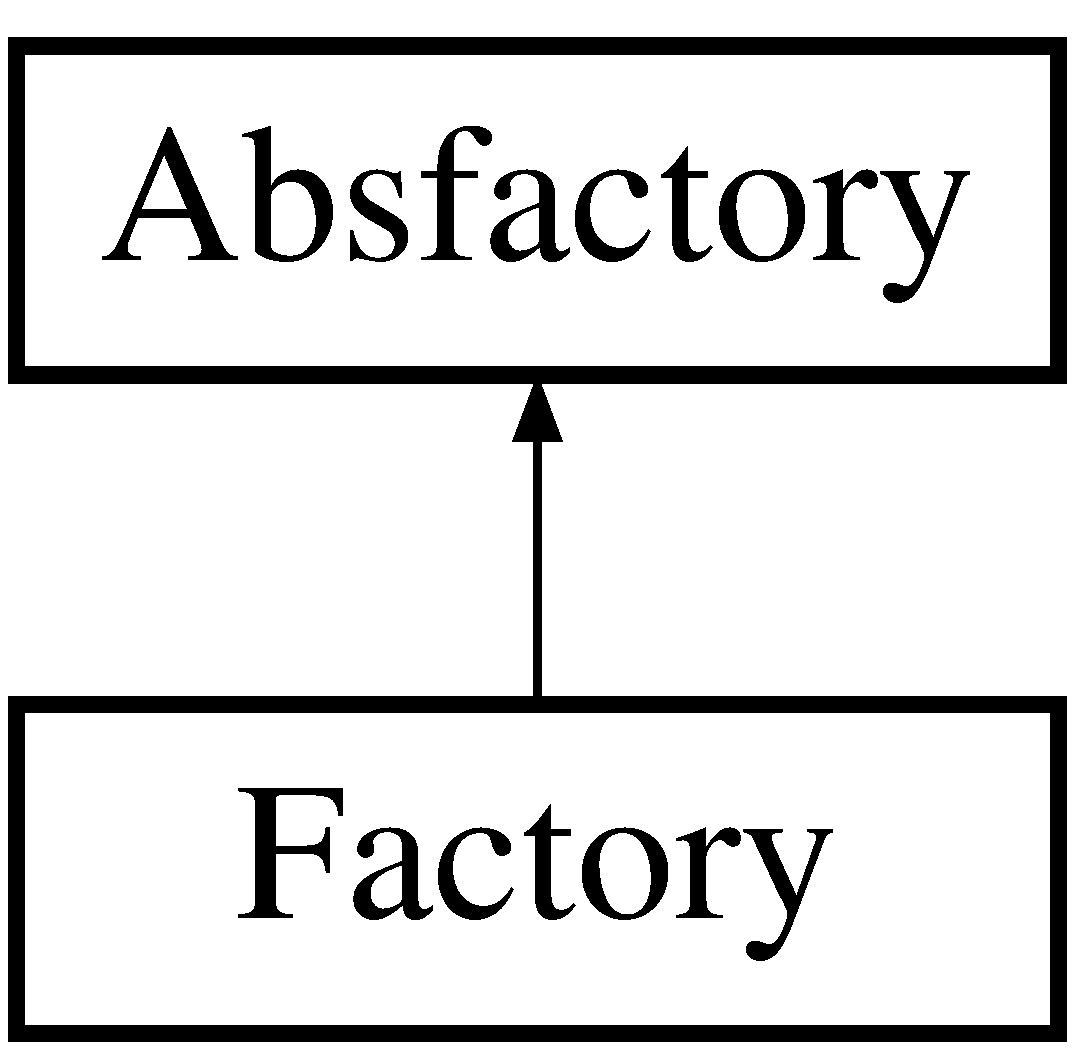
\includegraphics[height=2.000000cm]{class_absfactory}
\end{center}
\end{figure}
\subsection*{Public Member Functions}
\begin{DoxyCompactItemize}
\item 
\mbox{\Hypertarget{class_absfactory_a7a98426403d36416980f90323691df10}\label{class_absfactory_a7a98426403d36416980f90323691df10}} 
virtual \mbox{\hyperlink{classpool_table}{pool\+Table}} $\ast$ \mbox{\hyperlink{class_absfactory_a7a98426403d36416980f90323691df10}{create\+Table}} (double xsize=100, double ysize=100, string color=\char`\"{}white\char`\"{}, double fri=0)=0
\begin{DoxyCompactList}\small\item\em a method of creating table object. \end{DoxyCompactList}\item 
\mbox{\Hypertarget{class_absfactory_a69280d7c37d809c84b326f29f36b2804}\label{class_absfactory_a69280d7c37d809c84b326f29f36b2804}} 
virtual \mbox{\hyperlink{classpool_ball}{pool\+Ball}} $\ast$ \mbox{\hyperlink{class_absfactory_a69280d7c37d809c84b326f29f36b2804}{create\+Ball}} (\mbox{\hyperlink{class_coordinate}{Coordinate}} coordinate, double radius, string color, double mass, \mbox{\hyperlink{class_velocity}{Velocity}} velocity)=0
\begin{DoxyCompactList}\small\item\em a method of creating ball obejct. \end{DoxyCompactList}\end{DoxyCompactItemize}


\subsection{Detailed Description}
It is the abstract factory and named \mbox{\hyperlink{class_absfactory}{Absfactory}} as a part of abstract factory design pattern structure. 

The documentation for this class was generated from the following file\+:\begin{DoxyCompactItemize}
\item 
factory.\+h\end{DoxyCompactItemize}

\hypertarget{classball}{}\section{ball Class Reference}
\label{classball}\index{ball@{ball}}
Inheritance diagram for ball\+:\begin{figure}[H]
\begin{center}
\leavevmode
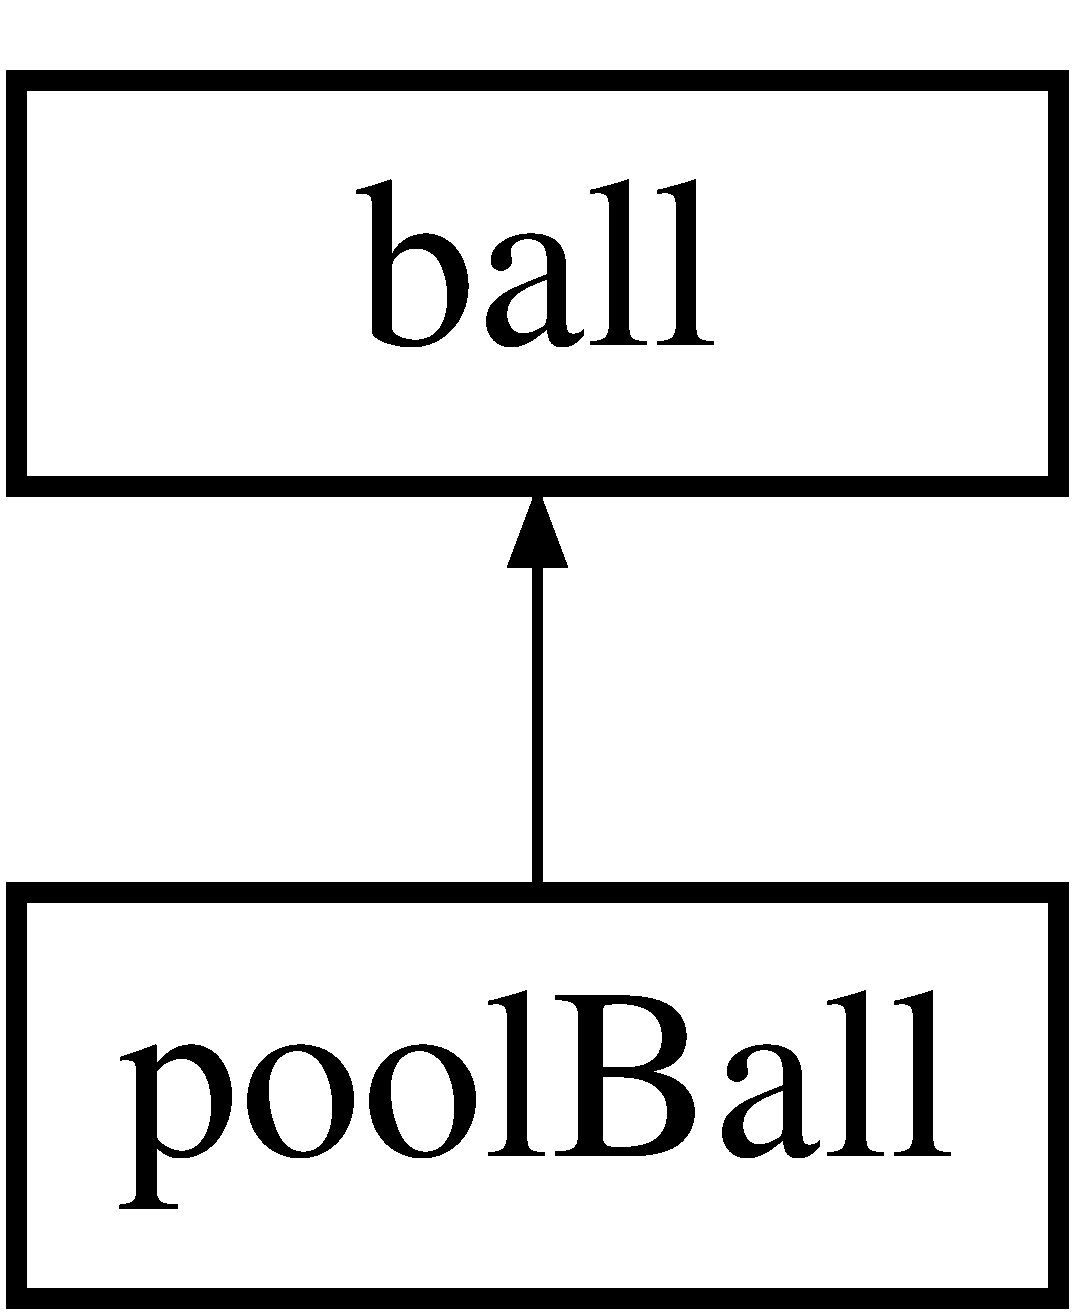
\includegraphics[height=2.000000cm]{classball}
\end{center}
\end{figure}


The documentation for this class was generated from the following file\+:\begin{DoxyCompactItemize}
\item 
product.\+h\end{DoxyCompactItemize}

\hypertarget{class_coordinate}{}\section{Coordinate Class Reference}
\label{class_coordinate}\index{Coordinate@{Coordinate}}


{\ttfamily \#include $<$coordinate.\+h$>$}

\subsection*{Public Member Functions}
\begin{DoxyCompactItemize}
\item 
\mbox{\Hypertarget{class_coordinate_ac100ccbb6ae098e04a33d09695e37c27}\label{class_coordinate_ac100ccbb6ae098e04a33d09695e37c27}} 
{\bfseries Coordinate} (double x\+Coordinate, double y\+Coordinate, double frame\+Height)
\item 
\mbox{\Hypertarget{class_coordinate_ae29b2ae00ef197df611c9445b45a3e62}\label{class_coordinate_ae29b2ae00ef197df611c9445b45a3e62}} 
double \mbox{\hyperlink{class_coordinate_ae29b2ae00ef197df611c9445b45a3e62}{get\+Qt\+Rendering\+X\+Coordinate}} ()
\begin{DoxyCompactList}\small\item\em get x coordinate \end{DoxyCompactList}\item 
\mbox{\Hypertarget{class_coordinate_a04a4454970075707e98fa24abcc7fd72}\label{class_coordinate_a04a4454970075707e98fa24abcc7fd72}} 
double \mbox{\hyperlink{class_coordinate_a04a4454970075707e98fa24abcc7fd72}{get\+Qt\+Rendering\+Y\+Coordinate}} ()
\begin{DoxyCompactList}\small\item\em get y coordinate \end{DoxyCompactList}\item 
\mbox{\Hypertarget{class_coordinate_a663c89f2bcdb4efb9416df4a42d95eb5}\label{class_coordinate_a663c89f2bcdb4efb9416df4a42d95eb5}} 
void \mbox{\hyperlink{class_coordinate_a663c89f2bcdb4efb9416df4a42d95eb5}{change\+In\+X\+Coordinate}} (double change)
\begin{DoxyCompactList}\small\item\em change x coordinate by increasing the value of change \end{DoxyCompactList}\item 
\mbox{\Hypertarget{class_coordinate_a4a7edaafaee90471fa91f9e4720960a0}\label{class_coordinate_a4a7edaafaee90471fa91f9e4720960a0}} 
void \mbox{\hyperlink{class_coordinate_a4a7edaafaee90471fa91f9e4720960a0}{change\+In\+Y\+Coordinate}} (double change)
\begin{DoxyCompactList}\small\item\em change y coordinate by increasing the value of change \end{DoxyCompactList}\item 
\mbox{\Hypertarget{class_coordinate_a3d903978af2a8f566328f5ef25b09a0d}\label{class_coordinate_a3d903978af2a8f566328f5ef25b09a0d}} 
void \mbox{\hyperlink{class_coordinate_a3d903978af2a8f566328f5ef25b09a0d}{change\+Frame\+Height}} (double change)
\begin{DoxyCompactList}\small\item\em change frame height by increasing the value of change \end{DoxyCompactList}\item 
\mbox{\Hypertarget{class_coordinate_a3fa2a351ac8952bce7574aabb42b05e0}\label{class_coordinate_a3fa2a351ac8952bce7574aabb42b05e0}} 
void \mbox{\hyperlink{class_coordinate_a3fa2a351ac8952bce7574aabb42b05e0}{set\+Y\+Coordinate\+To\+Zero}} (double offset)
\begin{DoxyCompactList}\small\item\em set y to offset \end{DoxyCompactList}\item 
\mbox{\Hypertarget{class_coordinate_a9344e8989dada3bf791b5dde42544fa3}\label{class_coordinate_a9344e8989dada3bf791b5dde42544fa3}} 
void \mbox{\hyperlink{class_coordinate_a9344e8989dada3bf791b5dde42544fa3}{set\+X\+Coordinate\+To\+Zero}} (double offset)
\begin{DoxyCompactList}\small\item\em set x to offset \end{DoxyCompactList}\item 
\mbox{\Hypertarget{class_coordinate_a9263be4ba7bf18ab8a67e1aafdf6dc09}\label{class_coordinate_a9263be4ba7bf18ab8a67e1aafdf6dc09}} 
double \mbox{\hyperlink{class_coordinate_a9263be4ba7bf18ab8a67e1aafdf6dc09}{get\+Frame\+Height}} ()
\begin{DoxyCompactList}\small\item\em get x coordnate \end{DoxyCompactList}\end{DoxyCompactItemize}


\subsection{Detailed Description}
I set coordinate of all elements of pool game as a class named \mbox{\hyperlink{class_coordinate}{Coordinate}}, it has two memeber variable for x, y. And some methods for modifying and getting x, y. It is used in pool ball class and pool table class. 

The documentation for this class was generated from the following files\+:\begin{DoxyCompactItemize}
\item 
coordinate.\+h\item 
coordinate.\+cpp\end{DoxyCompactItemize}

\hypertarget{class_dialog}{}\section{Dialog Class Reference}
\label{class_dialog}\index{Dialog@{Dialog}}
Inheritance diagram for Dialog\+:\begin{figure}[H]
\begin{center}
\leavevmode
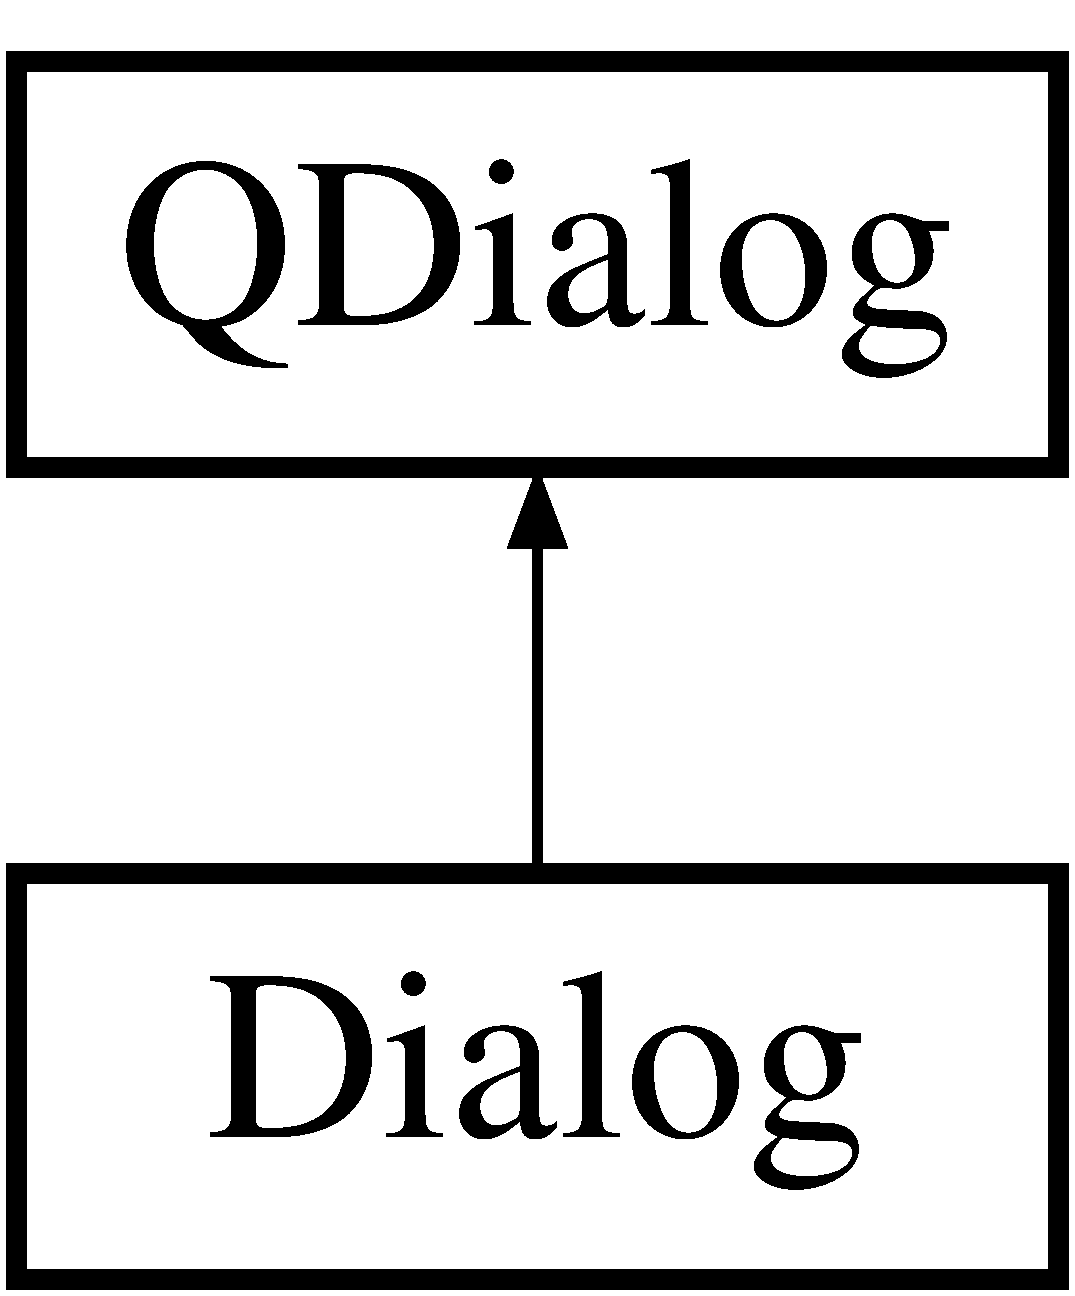
\includegraphics[height=2.000000cm]{class_dialog}
\end{center}
\end{figure}
\subsection*{Public Slots}
\begin{DoxyCompactItemize}
\item 
\mbox{\Hypertarget{class_dialog_a8bc4fe3b0cc12033369b49eab8751e14}\label{class_dialog_a8bc4fe3b0cc12033369b49eab8751e14}} 
void \mbox{\hyperlink{class_dialog_a8bc4fe3b0cc12033369b49eab8751e14}{next\+Frame}} ()
\begin{DoxyCompactList}\small\item\em To update. \end{DoxyCompactList}\end{DoxyCompactItemize}
\subsection*{Public Member Functions}
\begin{DoxyCompactItemize}
\item 
\mbox{\Hypertarget{class_dialog_a877ced4e29e3638b2f8925a954852ca0}\label{class_dialog_a877ced4e29e3638b2f8925a954852ca0}} 
{\bfseries Dialog} (\mbox{\hyperlink{classpool_game}{pool\+Game}} $\ast$pg, Q\+Widget $\ast$parent=0)
\end{DoxyCompactItemize}
\subsection*{Protected Member Functions}
\begin{DoxyCompactItemize}
\item 
\mbox{\Hypertarget{class_dialog_ac761f05fce616d76acf0612370b857ad}\label{class_dialog_ac761f05fce616d76acf0612370b857ad}} 
void \mbox{\hyperlink{class_dialog_ac761f05fce616d76acf0612370b857ad}{paint\+Event}} (Q\+Paint\+Event $\ast$event)
\begin{DoxyCompactList}\small\item\em To paint. \end{DoxyCompactList}\end{DoxyCompactItemize}


The documentation for this class was generated from the following files\+:\begin{DoxyCompactItemize}
\item 
dialog.\+h\item 
dialog.\+cpp\end{DoxyCompactItemize}

\hypertarget{classdirector}{}\section{director Class Reference}
\label{classdirector}\index{director@{director}}
\subsection*{Public Member Functions}
\begin{DoxyCompactItemize}
\item 
\mbox{\Hypertarget{classdirector_aec973b938b96f5e0a2a1995a2204e66a}\label{classdirector_aec973b938b96f5e0a2a1995a2204e66a}} 
{\bfseries director} (\mbox{\hyperlink{classmanufacturer}{manufacturer}} $\ast$builder)
\item 
\mbox{\Hypertarget{classdirector_aa322af5ca7653c81caec2d6e0cbc37d8}\label{classdirector_aa322af5ca7653c81caec2d6e0cbc37d8}} 
\mbox{\hyperlink{classpool_game}{pool\+Game}} $\ast$ {\bfseries construct} (int n, \mbox{\hyperlink{classpool_table}{pool\+Table}} t\+\_\+table, vector$<$ \mbox{\hyperlink{classpool_ball}{pool\+Ball}} $>$ t\+\_\+balls)
\end{DoxyCompactItemize}


The documentation for this class was generated from the following file\+:\begin{DoxyCompactItemize}
\item 
main.\+cpp\end{DoxyCompactItemize}

\hypertarget{class_factory}{}\section{Factory Class Reference}
\label{class_factory}\index{Factory@{Factory}}


{\ttfamily \#include $<$concretefactory.\+h$>$}

Inheritance diagram for Factory\+:\begin{figure}[H]
\begin{center}
\leavevmode
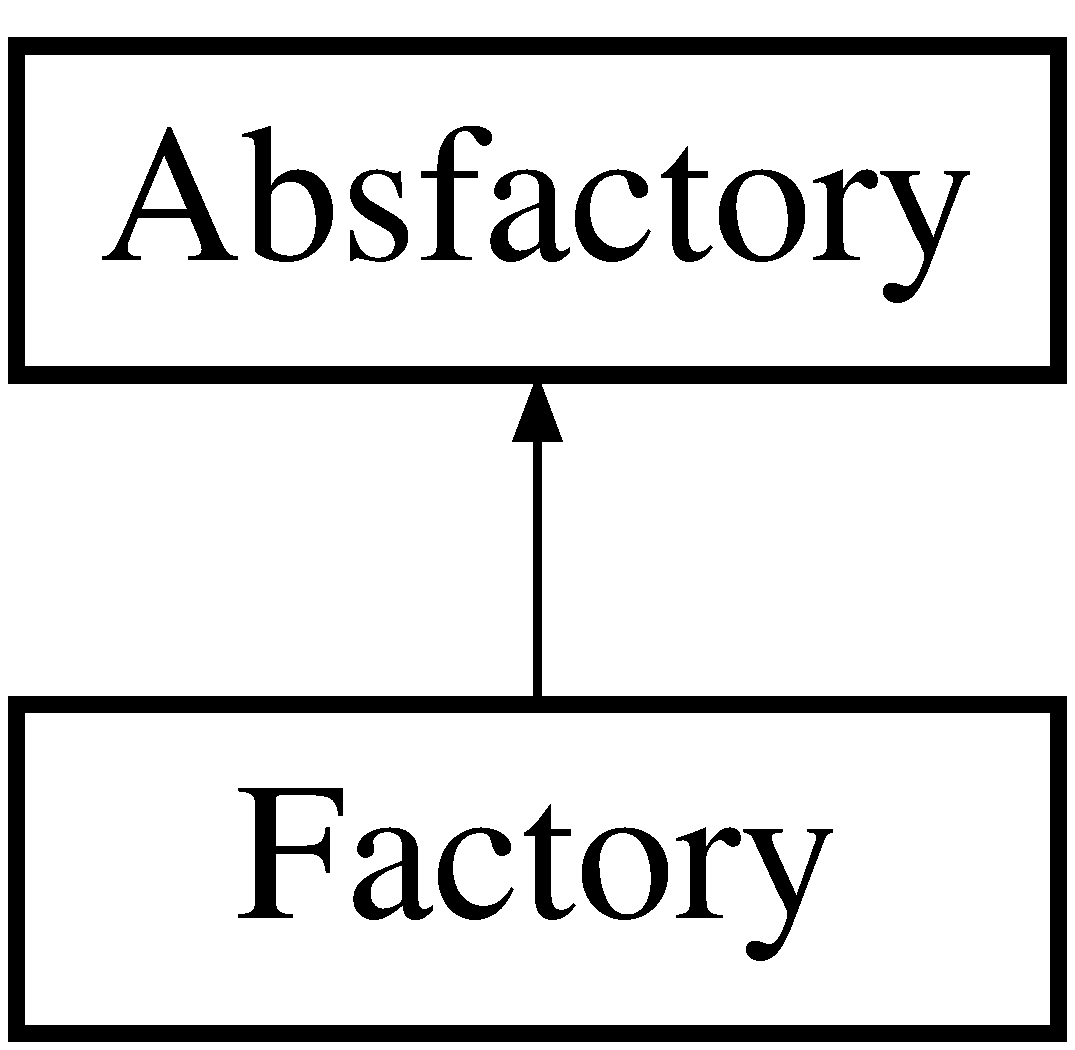
\includegraphics[height=2.000000cm]{class_factory}
\end{center}
\end{figure}
\subsection*{Public Member Functions}
\begin{DoxyCompactItemize}
\item 
\mbox{\Hypertarget{class_factory_ab814feb40a237a087bbf1b1c4c128dc6}\label{class_factory_ab814feb40a237a087bbf1b1c4c128dc6}} 
\mbox{\hyperlink{classpool_table}{pool\+Table}} $\ast$ \mbox{\hyperlink{class_factory_ab814feb40a237a087bbf1b1c4c128dc6}{create\+Table}} (double xsize=100, double ysize=100, string color=\char`\"{}white\char`\"{}, double fri=0)
\begin{DoxyCompactList}\small\item\em a method of creating table object. \end{DoxyCompactList}\item 
\mbox{\Hypertarget{class_factory_a30decbb04d0365e543bd2131eb3c9877}\label{class_factory_a30decbb04d0365e543bd2131eb3c9877}} 
\mbox{\hyperlink{classpool_ball}{pool\+Ball}} $\ast$ \mbox{\hyperlink{class_factory_a30decbb04d0365e543bd2131eb3c9877}{create\+Ball}} (\mbox{\hyperlink{class_coordinate}{Coordinate}} coordinate, double radius, string color, double mass, \mbox{\hyperlink{class_velocity}{Velocity}} velocity)
\begin{DoxyCompactList}\small\item\em a method of creating ball obejct. \end{DoxyCompactList}\end{DoxyCompactItemize}


\subsection{Detailed Description}
It is concrete factory derived from abstract factory, and it will be used for prduction. 

The documentation for this class was generated from the following files\+:\begin{DoxyCompactItemize}
\item 
concretefactory.\+h\item 
concretefactory.\+cpp\end{DoxyCompactItemize}

\hypertarget{classmanufacturer}{}\section{manufacturer Class Reference}
\label{classmanufacturer}\index{manufacturer@{manufacturer}}


{\ttfamily \#include $<$builder.\+h$>$}

Inheritance diagram for manufacturer\+:\begin{figure}[H]
\begin{center}
\leavevmode
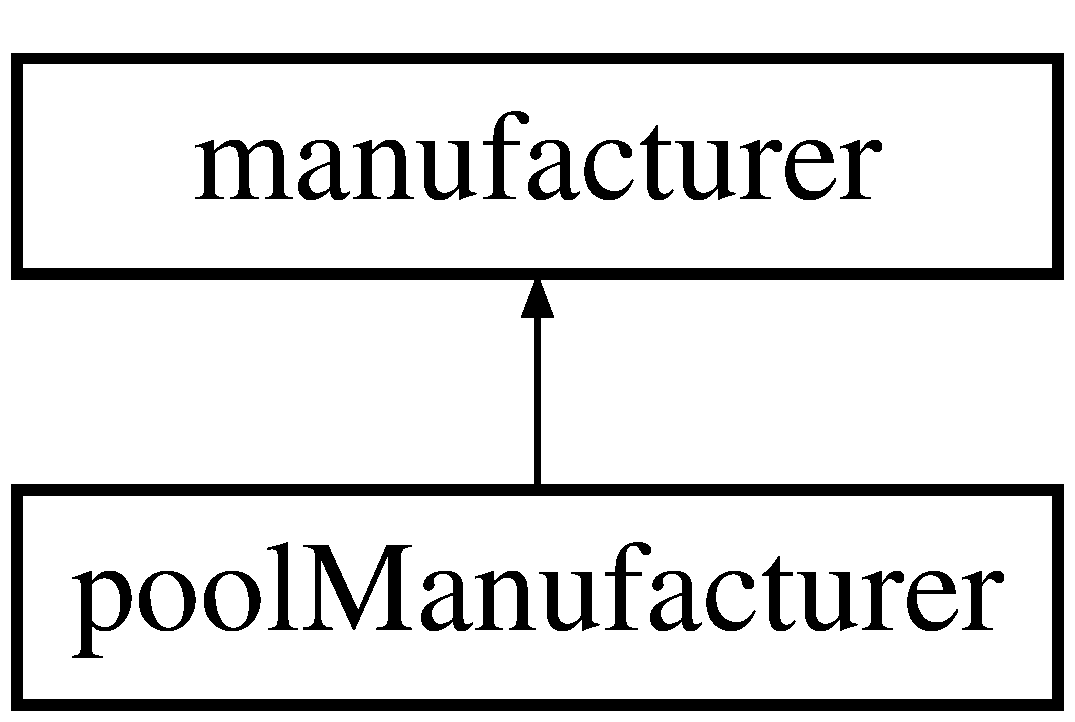
\includegraphics[height=2.000000cm]{classmanufacturer}
\end{center}
\end{figure}
\subsection*{Public Member Functions}
\begin{DoxyCompactItemize}
\item 
\mbox{\Hypertarget{classmanufacturer_a9b3efc9046298f34d56bfa66b89ef168}\label{classmanufacturer_a9b3efc9046298f34d56bfa66b89ef168}} 
virtual \mbox{\hyperlink{classpool_table}{pool\+Table}} $\ast$ \mbox{\hyperlink{classmanufacturer_a9b3efc9046298f34d56bfa66b89ef168}{build\+Table}} (double xsize, double ysize, string color, double fri)=0
\begin{DoxyCompactList}\small\item\em a method of building table \end{DoxyCompactList}\item 
\mbox{\Hypertarget{classmanufacturer_a46701478dc4d2fa5c9bbe5257d19d26c}\label{classmanufacturer_a46701478dc4d2fa5c9bbe5257d19d26c}} 
virtual \mbox{\hyperlink{classpool_ball}{pool\+Ball}} $\ast$ \mbox{\hyperlink{classmanufacturer_a46701478dc4d2fa5c9bbe5257d19d26c}{build\+Ball}} (\mbox{\hyperlink{class_coordinate}{Coordinate}} coordinate, double radius, string color, double mass, \mbox{\hyperlink{class_velocity}{Velocity}} velocity)=0
\begin{DoxyCompactList}\small\item\em a method of buidling table \end{DoxyCompactList}\item 
\mbox{\Hypertarget{classmanufacturer_a16f727b4433ba779beb2ce9b67a2087c}\label{classmanufacturer_a16f727b4433ba779beb2ce9b67a2087c}} 
virtual \mbox{\hyperlink{classpool_game}{pool\+Game}} $\ast$ {\bfseries get\+Pool} ()=0
\end{DoxyCompactItemize}
\subsection*{Public Attributes}
\begin{DoxyCompactItemize}
\item 
\mbox{\Hypertarget{classmanufacturer_ac73ee10721c5d41dc1f2d07128ea33d9}\label{classmanufacturer_ac73ee10721c5d41dc1f2d07128ea33d9}} 
\mbox{\hyperlink{class_factory}{Factory}} \mbox{\hyperlink{classmanufacturer_ac73ee10721c5d41dc1f2d07128ea33d9}{factory}}
\begin{DoxyCompactList}\small\item\em using factory in builder \end{DoxyCompactList}\end{DoxyCompactItemize}


\subsection{Detailed Description}
this file is the abstract builder, which is the manufacturer. 

The documentation for this class was generated from the following file\+:\begin{DoxyCompactItemize}
\item 
builder.\+h\end{DoxyCompactItemize}

\hypertarget{classpool_ball}{}\section{pool\+Ball Class Reference}
\label{classpool_ball}\index{pool\+Ball@{pool\+Ball}}
Inheritance diagram for pool\+Ball\+:\begin{figure}[H]
\begin{center}
\leavevmode
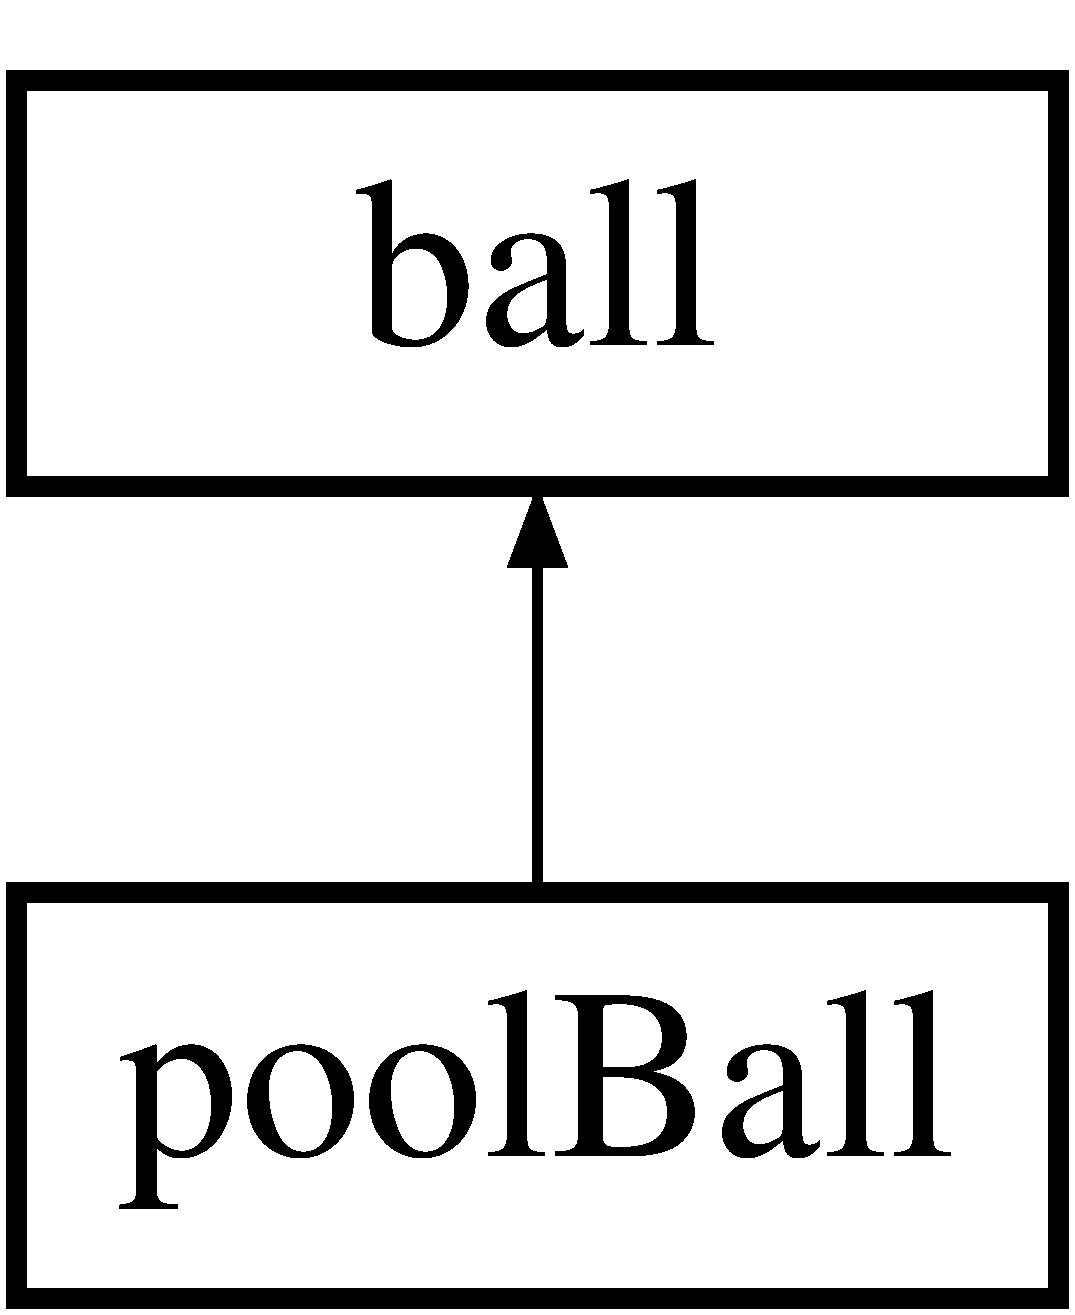
\includegraphics[height=2.000000cm]{classpool_ball}
\end{center}
\end{figure}
\subsection*{Public Member Functions}
\begin{DoxyCompactItemize}
\item 
\mbox{\Hypertarget{classpool_ball_ab6d6082e1368588d31bb3ea111121525}\label{classpool_ball_ab6d6082e1368588d31bb3ea111121525}} 
{\bfseries pool\+Ball} (\mbox{\hyperlink{class_coordinate}{Coordinate}} coordinate, double radius, string color, double mass, \mbox{\hyperlink{class_velocity}{Velocity}} velocity)
\item 
void \mbox{\hyperlink{classpool_ball_ab98b836bfc2de5d1573a6f015614da75}{change\+VX}} (double change)
\item 
void \mbox{\hyperlink{classpool_ball_af0816c210e83ac30c1cedde19fd92c4a}{change\+VY}} (double change)
\item 
\mbox{\Hypertarget{classpool_ball_a8ada7169ca79112aca09cd9434c52dba}\label{classpool_ball_a8ada7169ca79112aca09cd9434c52dba}} 
\mbox{\hyperlink{class_coordinate}{Coordinate}} {\bfseries getcoordinate} ()
\item 
\mbox{\Hypertarget{classpool_ball_a0f57c701684d7c8bb6cdb584c328881c}\label{classpool_ball_a0f57c701684d7c8bb6cdb584c328881c}} 
double {\bfseries getradius} ()
\item 
\mbox{\Hypertarget{classpool_ball_a07bcecd4fe38d1363f7cf08359183f24}\label{classpool_ball_a07bcecd4fe38d1363f7cf08359183f24}} 
string {\bfseries getcolor} ()
\item 
\mbox{\Hypertarget{classpool_ball_ab1acec22de9a8d4de61ffd8efacd4076}\label{classpool_ball_ab1acec22de9a8d4de61ffd8efacd4076}} 
double {\bfseries getmass} ()
\item 
\mbox{\Hypertarget{classpool_ball_a5ff8845804ee770cfb52e20bb17e7f4b}\label{classpool_ball_a5ff8845804ee770cfb52e20bb17e7f4b}} 
\mbox{\hyperlink{class_velocity}{Velocity}} {\bfseries getvelocity} ()
\item 
void \mbox{\hyperlink{classpool_ball_a62f83890e97cd5b40f97103e835e38da}{is\+Collision\+Wall}} (Q\+Painter \&painter, unsigned int time, double x, double y, double fri)
\end{DoxyCompactItemize}


\subsection{Member Function Documentation}
\mbox{\Hypertarget{classpool_ball_ab98b836bfc2de5d1573a6f015614da75}\label{classpool_ball_ab98b836bfc2de5d1573a6f015614da75}} 
\index{pool\+Ball@{pool\+Ball}!change\+VX@{change\+VX}}
\index{change\+VX@{change\+VX}!pool\+Ball@{pool\+Ball}}
\subsubsection{\texorpdfstring{change\+V\+X()}{changeVX()}}
{\footnotesize\ttfamily void pool\+Ball\+::change\+VX (\begin{DoxyParamCaption}\item[{double}]{change }\end{DoxyParamCaption})\hspace{0.3cm}{\ttfamily [inline]}}


\begin{DoxyParams}{Parameters}
{\em change} & change the value of x velocity \\
\hline
\end{DoxyParams}
\mbox{\Hypertarget{classpool_ball_af0816c210e83ac30c1cedde19fd92c4a}\label{classpool_ball_af0816c210e83ac30c1cedde19fd92c4a}} 
\index{pool\+Ball@{pool\+Ball}!change\+VY@{change\+VY}}
\index{change\+VY@{change\+VY}!pool\+Ball@{pool\+Ball}}
\subsubsection{\texorpdfstring{change\+V\+Y()}{changeVY()}}
{\footnotesize\ttfamily void pool\+Ball\+::change\+VY (\begin{DoxyParamCaption}\item[{double}]{change }\end{DoxyParamCaption})\hspace{0.3cm}{\ttfamily [inline]}}


\begin{DoxyParams}{Parameters}
{\em change} & change the value of y velocity \\
\hline
\end{DoxyParams}
\mbox{\Hypertarget{classpool_ball_a62f83890e97cd5b40f97103e835e38da}\label{classpool_ball_a62f83890e97cd5b40f97103e835e38da}} 
\index{pool\+Ball@{pool\+Ball}!is\+Collision\+Wall@{is\+Collision\+Wall}}
\index{is\+Collision\+Wall@{is\+Collision\+Wall}!pool\+Ball@{pool\+Ball}}
\subsubsection{\texorpdfstring{is\+Collision\+Wall()}{isCollisionWall()}}
{\footnotesize\ttfamily void pool\+Ball\+::is\+Collision\+Wall (\begin{DoxyParamCaption}\item[{Q\+Painter \&}]{painter,  }\item[{unsigned int}]{time,  }\item[{double}]{x,  }\item[{double}]{y,  }\item[{double}]{fri }\end{DoxyParamCaption})\hspace{0.3cm}{\ttfamily [inline]}}


\begin{DoxyParams}{Parameters}
{\em fri} & check the ball-\/wall collision and calculate velocity change and cooridnate change \\
\hline
\end{DoxyParams}


The documentation for this class was generated from the following file\+:\begin{DoxyCompactItemize}
\item 
product.\+h\end{DoxyCompactItemize}

\hypertarget{classpool_game}{}\section{pool\+Game Class Reference}
\label{classpool_game}\index{pool\+Game@{pool\+Game}}
\subsection*{Public Member Functions}
\begin{DoxyCompactItemize}
\item 
void \mbox{\hyperlink{classpool_game_a2f5550cf716aacfd50995fb73cb6602f}{add\+Table}} (\mbox{\hyperlink{classpool_table}{pool\+Table}} $\ast$\mbox{\hyperlink{classtable}{table}})
\item 
void \mbox{\hyperlink{classpool_game_a15f39114d5ee90d98521c01ab0f61f93}{add\+Ball}} (\mbox{\hyperlink{classpool_ball}{pool\+Ball}} $\ast$\mbox{\hyperlink{classball}{ball}})
\item 
\mbox{\Hypertarget{classpool_game_a3493923000e44ff21712f1fbb0f159f6}\label{classpool_game_a3493923000e44ff21712f1fbb0f159f6}} 
\mbox{\hyperlink{classpool_table}{pool\+Table}} $\ast$ {\bfseries getpooltable} ()
\item 
\mbox{\hyperlink{classpool_ball}{pool\+Ball}} $\ast$ \mbox{\hyperlink{classpool_game_ae1c3bfe159dca6d35cf447ba634fbfea}{get\+One\+Poolball}} (int n)
\item 
\mbox{\Hypertarget{classpool_game_a7fbf9126542caa46842d3ece276cb014}\label{classpool_game_a7fbf9126542caa46842d3ece276cb014}} 
std\+::vector$<$ \mbox{\hyperlink{classpool_ball}{pool\+Ball}} $\ast$ $>$ {\bfseries getpool\+Balls} ()
\item 
bool \mbox{\hyperlink{classpool_game_a171207b2803656237a241d30843bf883}{is\+Ball\+Collision}} (\mbox{\hyperlink{classpool_ball}{pool\+Ball}} $\ast$A, \mbox{\hyperlink{classpool_ball}{pool\+Ball}} $\ast$B)
\item 
void \mbox{\hyperlink{classpool_game_a2b907f407d0de6644271b4e1a66a4f3c}{Collision\+Ball}} (\mbox{\hyperlink{classpool_ball}{pool\+Ball}} $\ast$A, \mbox{\hyperlink{classpool_ball}{pool\+Ball}} $\ast$B)
\end{DoxyCompactItemize}


\subsection{Member Function Documentation}
\mbox{\Hypertarget{classpool_game_a15f39114d5ee90d98521c01ab0f61f93}\label{classpool_game_a15f39114d5ee90d98521c01ab0f61f93}} 
\index{pool\+Game@{pool\+Game}!add\+Ball@{add\+Ball}}
\index{add\+Ball@{add\+Ball}!pool\+Game@{pool\+Game}}
\subsubsection{\texorpdfstring{add\+Ball()}{addBall()}}
{\footnotesize\ttfamily void pool\+Game\+::add\+Ball (\begin{DoxyParamCaption}\item[{\mbox{\hyperlink{classpool_ball}{pool\+Ball}} $\ast$}]{ball }\end{DoxyParamCaption})\hspace{0.3cm}{\ttfamily [inline]}}


\begin{DoxyParams}{Parameters}
{\em ball} & add a pool ba;; \\
\hline
\end{DoxyParams}
\mbox{\Hypertarget{classpool_game_a2f5550cf716aacfd50995fb73cb6602f}\label{classpool_game_a2f5550cf716aacfd50995fb73cb6602f}} 
\index{pool\+Game@{pool\+Game}!add\+Table@{add\+Table}}
\index{add\+Table@{add\+Table}!pool\+Game@{pool\+Game}}
\subsubsection{\texorpdfstring{add\+Table()}{addTable()}}
{\footnotesize\ttfamily void pool\+Game\+::add\+Table (\begin{DoxyParamCaption}\item[{\mbox{\hyperlink{classpool_table}{pool\+Table}} $\ast$}]{table }\end{DoxyParamCaption})\hspace{0.3cm}{\ttfamily [inline]}}


\begin{DoxyParams}{Parameters}
{\em table} & add a pool table \\
\hline
\end{DoxyParams}
\mbox{\Hypertarget{classpool_game_a2b907f407d0de6644271b4e1a66a4f3c}\label{classpool_game_a2b907f407d0de6644271b4e1a66a4f3c}} 
\index{pool\+Game@{pool\+Game}!Collision\+Ball@{Collision\+Ball}}
\index{Collision\+Ball@{Collision\+Ball}!pool\+Game@{pool\+Game}}
\subsubsection{\texorpdfstring{Collision\+Ball()}{CollisionBall()}}
{\footnotesize\ttfamily void pool\+Game\+::\+Collision\+Ball (\begin{DoxyParamCaption}\item[{\mbox{\hyperlink{classpool_ball}{pool\+Ball}} $\ast$}]{A,  }\item[{\mbox{\hyperlink{classpool_ball}{pool\+Ball}} $\ast$}]{B }\end{DoxyParamCaption})\hspace{0.3cm}{\ttfamily [inline]}}


\begin{DoxyParams}{Parameters}
{\em B} & calculate the velocity and cooridnate change of two collided balls \\
\hline
\end{DoxyParams}
\mbox{\Hypertarget{classpool_game_ae1c3bfe159dca6d35cf447ba634fbfea}\label{classpool_game_ae1c3bfe159dca6d35cf447ba634fbfea}} 
\index{pool\+Game@{pool\+Game}!get\+One\+Poolball@{get\+One\+Poolball}}
\index{get\+One\+Poolball@{get\+One\+Poolball}!pool\+Game@{pool\+Game}}
\subsubsection{\texorpdfstring{get\+One\+Poolball()}{getOnePoolball()}}
{\footnotesize\ttfamily \mbox{\hyperlink{classpool_ball}{pool\+Ball}}$\ast$ pool\+Game\+::get\+One\+Poolball (\begin{DoxyParamCaption}\item[{int}]{n }\end{DoxyParamCaption})\hspace{0.3cm}{\ttfamily [inline]}}


\begin{DoxyParams}{Parameters}
{\em n} & get a pool ball from vector \\
\hline
\end{DoxyParams}
\mbox{\Hypertarget{classpool_game_a171207b2803656237a241d30843bf883}\label{classpool_game_a171207b2803656237a241d30843bf883}} 
\index{pool\+Game@{pool\+Game}!is\+Ball\+Collision@{is\+Ball\+Collision}}
\index{is\+Ball\+Collision@{is\+Ball\+Collision}!pool\+Game@{pool\+Game}}
\subsubsection{\texorpdfstring{is\+Ball\+Collision()}{isBallCollision()}}
{\footnotesize\ttfamily bool pool\+Game\+::is\+Ball\+Collision (\begin{DoxyParamCaption}\item[{\mbox{\hyperlink{classpool_ball}{pool\+Ball}} $\ast$}]{A,  }\item[{\mbox{\hyperlink{classpool_ball}{pool\+Ball}} $\ast$}]{B }\end{DoxyParamCaption})\hspace{0.3cm}{\ttfamily [inline]}}


\begin{DoxyParams}{Parameters}
{\em B} & check the ball-\/ball collision \\
\hline
\end{DoxyParams}


The documentation for this class was generated from the following file\+:\begin{DoxyCompactItemize}
\item 
product.\+h\end{DoxyCompactItemize}

\hypertarget{classpool_manufacturer}{}\section{pool\+Manufacturer Class Reference}
\label{classpool_manufacturer}\index{pool\+Manufacturer@{pool\+Manufacturer}}


{\ttfamily \#include $<$concretebuilder.\+h$>$}

Inheritance diagram for pool\+Manufacturer\+:\begin{figure}[H]
\begin{center}
\leavevmode
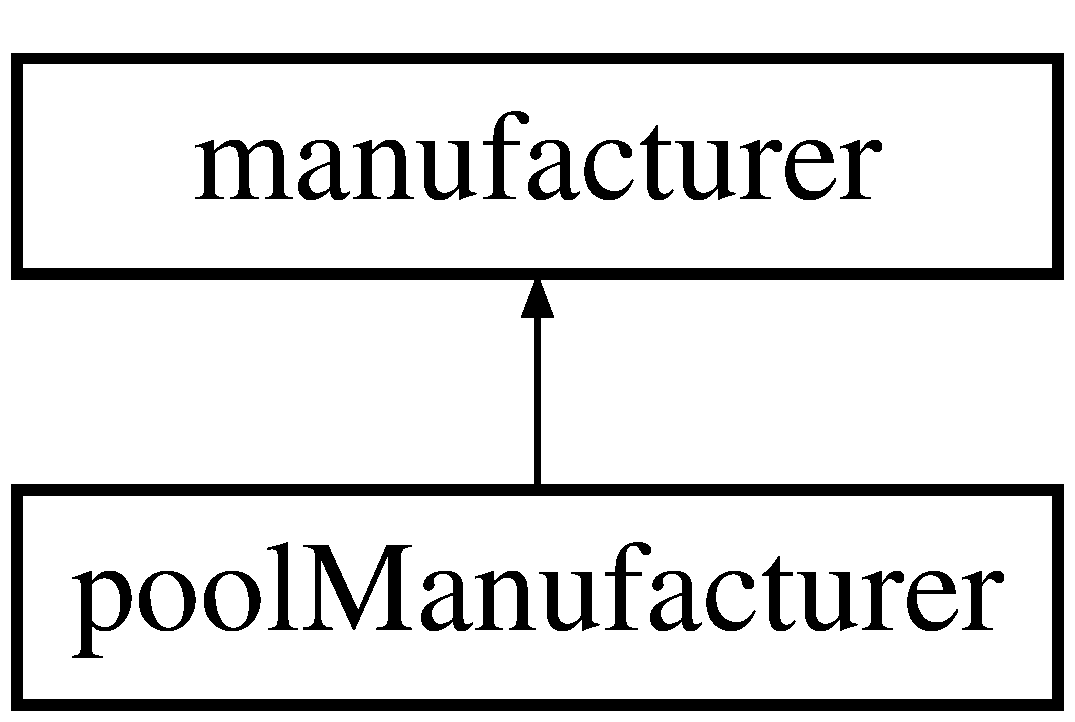
\includegraphics[height=2.000000cm]{classpool_manufacturer}
\end{center}
\end{figure}
\subsection*{Public Member Functions}
\begin{DoxyCompactItemize}
\item 
\mbox{\Hypertarget{classpool_manufacturer_a414e88ee1fd96bdf39525dae19ad147b}\label{classpool_manufacturer_a414e88ee1fd96bdf39525dae19ad147b}} 
virtual \mbox{\hyperlink{classpool_table}{pool\+Table}} $\ast$ \mbox{\hyperlink{classpool_manufacturer_a414e88ee1fd96bdf39525dae19ad147b}{build\+Table}} (double xsize, double ysize, string color, double fri)
\begin{DoxyCompactList}\small\item\em a method of building table \end{DoxyCompactList}\item 
\mbox{\Hypertarget{classpool_manufacturer_aa61c2bdc11ec1f78dae73cae74914f3c}\label{classpool_manufacturer_aa61c2bdc11ec1f78dae73cae74914f3c}} 
virtual \mbox{\hyperlink{classpool_ball}{pool\+Ball}} $\ast$ \mbox{\hyperlink{classpool_manufacturer_aa61c2bdc11ec1f78dae73cae74914f3c}{build\+Ball}} (\mbox{\hyperlink{class_coordinate}{Coordinate}} coordinate, double radius, string color, double mass, \mbox{\hyperlink{class_velocity}{Velocity}} velocity)
\begin{DoxyCompactList}\small\item\em a method of buidling table \end{DoxyCompactList}\item 
\mbox{\Hypertarget{classpool_manufacturer_a277aac732a912c5435a815ff4ec44d6c}\label{classpool_manufacturer_a277aac732a912c5435a815ff4ec44d6c}} 
virtual \mbox{\hyperlink{classpool_game}{pool\+Game}} $\ast$ {\bfseries get\+Pool} ()
\end{DoxyCompactItemize}
\subsection*{Additional Inherited Members}


\subsection{Detailed Description}
this file is the concrete buidler derived from abstract builder. The functions are from its base class. 

The documentation for this class was generated from the following files\+:\begin{DoxyCompactItemize}
\item 
concretebuilder.\+h\item 
concretebuilder.\+cpp\end{DoxyCompactItemize}

\hypertarget{classpool_table}{}\section{pool\+Table Class Reference}
\label{classpool_table}\index{pool\+Table@{pool\+Table}}
Inheritance diagram for pool\+Table\+:\begin{figure}[H]
\begin{center}
\leavevmode
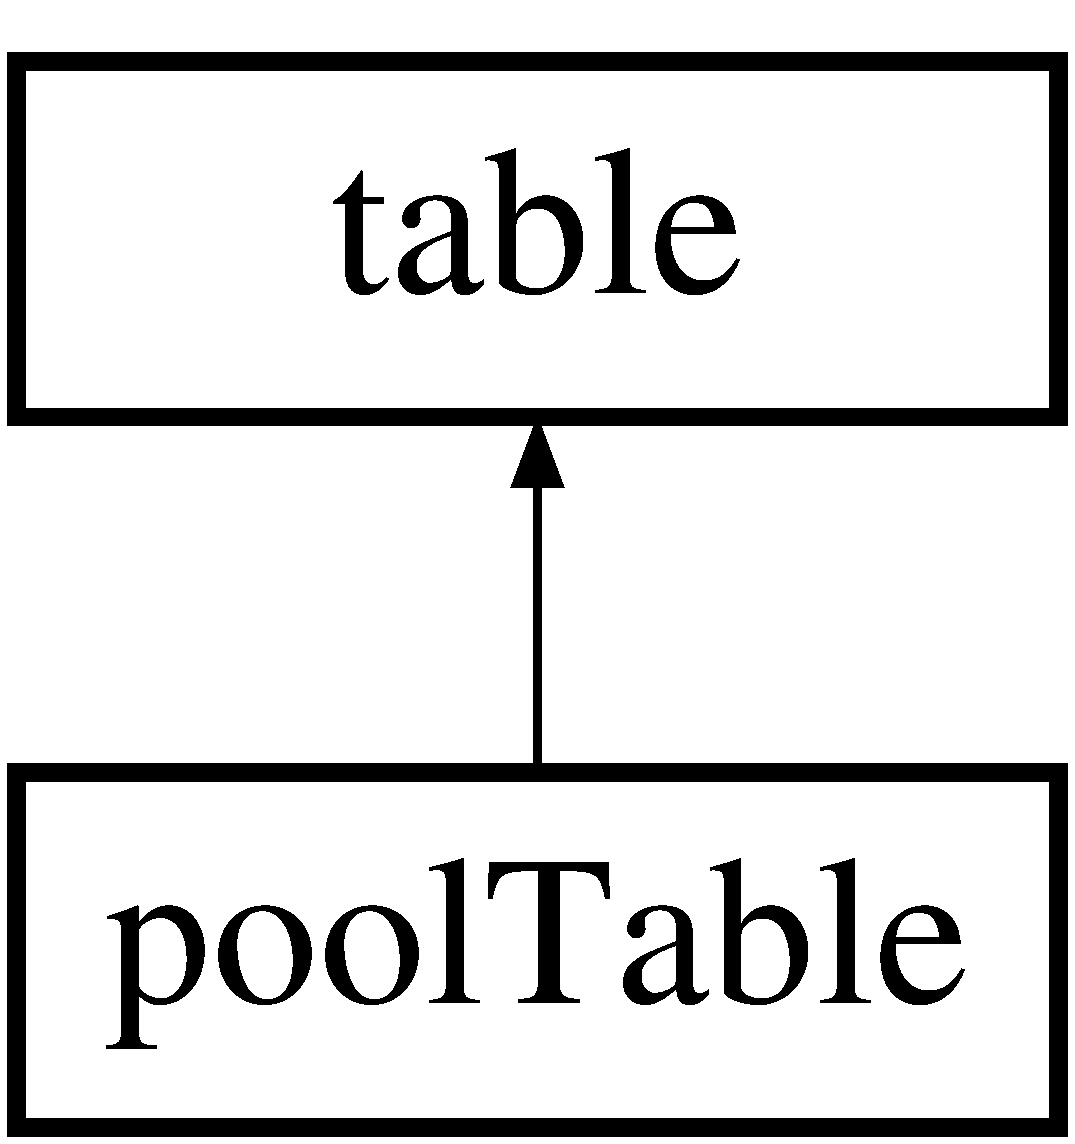
\includegraphics[height=2.000000cm]{classpool_table}
\end{center}
\end{figure}
\subsection*{Public Member Functions}
\begin{DoxyCompactItemize}
\item 
\mbox{\Hypertarget{classpool_table_a8e39cd90630d08a85d066ff01fab4a4e}\label{classpool_table_a8e39cd90630d08a85d066ff01fab4a4e}} 
{\bfseries pool\+Table} (double xsize=100, double ysize=100, string color=\char`\"{}white\char`\"{}, double friction=0)
\item 
\mbox{\Hypertarget{classpool_table_ae1daa626189b4eb4d0193cf34a06678f}\label{classpool_table_ae1daa626189b4eb4d0193cf34a06678f}} 
double {\bfseries getxsize} ()
\item 
\mbox{\Hypertarget{classpool_table_a360aab2e21ebbf489c378e05a032ef5e}\label{classpool_table_a360aab2e21ebbf489c378e05a032ef5e}} 
double {\bfseries getysize} ()
\item 
\mbox{\Hypertarget{classpool_table_ace06084f1066ca47a60915ae8589ae7e}\label{classpool_table_ace06084f1066ca47a60915ae8589ae7e}} 
double {\bfseries getfriction} ()
\item 
\mbox{\Hypertarget{classpool_table_a84be61ec08cc5688c25769fabd4c42c5}\label{classpool_table_a84be61ec08cc5688c25769fabd4c42c5}} 
string {\bfseries getcolor} ()
\end{DoxyCompactItemize}


The documentation for this class was generated from the following file\+:\begin{DoxyCompactItemize}
\item 
product.\+h\end{DoxyCompactItemize}

\hypertarget{classtable}{}\section{table Class Reference}
\label{classtable}\index{table@{table}}
Inheritance diagram for table\+:\begin{figure}[H]
\begin{center}
\leavevmode
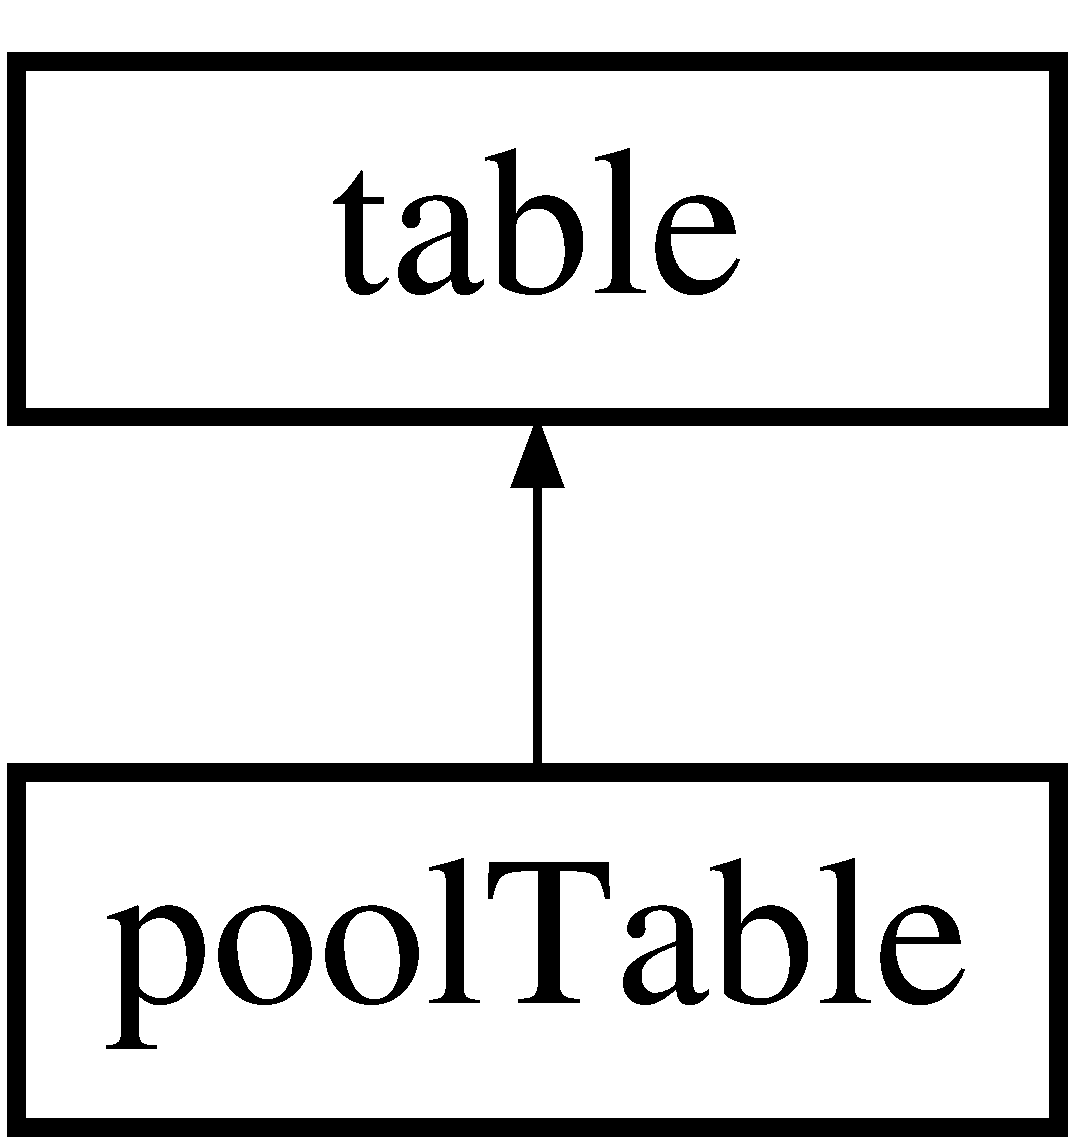
\includegraphics[height=2.000000cm]{classtable}
\end{center}
\end{figure}


The documentation for this class was generated from the following file\+:\begin{DoxyCompactItemize}
\item 
product.\+h\end{DoxyCompactItemize}

\hypertarget{class_velocity}{}\section{Velocity Class Reference}
\label{class_velocity}\index{Velocity@{Velocity}}


{\ttfamily \#include $<$velocity.\+h$>$}

\subsection*{Public Member Functions}
\begin{DoxyCompactItemize}
\item 
\mbox{\Hypertarget{class_velocity_ac7bb529bf5effe33ef79aef8acf34cc6}\label{class_velocity_ac7bb529bf5effe33ef79aef8acf34cc6}} 
{\bfseries Velocity} (double X\+Velocity, double Y\+Velocity)
\item 
\mbox{\Hypertarget{class_velocity_a38abeebec5b97d4f230c2a8995270621}\label{class_velocity_a38abeebec5b97d4f230c2a8995270621}} 
double \mbox{\hyperlink{class_velocity_a38abeebec5b97d4f230c2a8995270621}{get\+X\+Velocity}} ()
\begin{DoxyCompactList}\small\item\em get x velocity \end{DoxyCompactList}\item 
\mbox{\Hypertarget{class_velocity_a8318a85dc6732c0b896584df7be56775}\label{class_velocity_a8318a85dc6732c0b896584df7be56775}} 
double \mbox{\hyperlink{class_velocity_a8318a85dc6732c0b896584df7be56775}{get\+Y\+Velocity}} ()
\begin{DoxyCompactList}\small\item\em get y velocity \end{DoxyCompactList}\item 
\mbox{\Hypertarget{class_velocity_a441b45e36202610da088565d29d2bf88}\label{class_velocity_a441b45e36202610da088565d29d2bf88}} 
void \mbox{\hyperlink{class_velocity_a441b45e36202610da088565d29d2bf88}{change\+X\+Velocity}} (double change)
\begin{DoxyCompactList}\small\item\em change x velocity by increasing the value of change \end{DoxyCompactList}\item 
\mbox{\Hypertarget{class_velocity_a961a18e13d28c193049ab33a5b0a19b5}\label{class_velocity_a961a18e13d28c193049ab33a5b0a19b5}} 
void \mbox{\hyperlink{class_velocity_a961a18e13d28c193049ab33a5b0a19b5}{change\+Y\+Velocity}} (double change)
\begin{DoxyCompactList}\small\item\em change y velocity by increasing the value of change \end{DoxyCompactList}\item 
\mbox{\Hypertarget{class_velocity_a3a531f663840ebca863eee12edce6228}\label{class_velocity_a3a531f663840ebca863eee12edce6228}} 
void \mbox{\hyperlink{class_velocity_a3a531f663840ebca863eee12edce6228}{set\+X\+Offset}} ()
\begin{DoxyCompactList}\small\item\em set x velocity to 0 \end{DoxyCompactList}\item 
\mbox{\Hypertarget{class_velocity_a0f40761e683af492d86156110921edba}\label{class_velocity_a0f40761e683af492d86156110921edba}} 
void \mbox{\hyperlink{class_velocity_a0f40761e683af492d86156110921edba}{set\+Y\+Offset}} ()
\begin{DoxyCompactList}\small\item\em set y velocity to 0 \end{DoxyCompactList}\item 
\mbox{\Hypertarget{class_velocity_aca67fbc9b9aea417058bd305d75ef4ca}\label{class_velocity_aca67fbc9b9aea417058bd305d75ef4ca}} 
void \mbox{\hyperlink{class_velocity_aca67fbc9b9aea417058bd305d75ef4ca}{change\+X\+Direction}} ()
\begin{DoxyCompactList}\small\item\em change the direction of x velocity into opposite. \end{DoxyCompactList}\item 
\mbox{\Hypertarget{class_velocity_a943fd1b01734ee93fae40834f253ecce}\label{class_velocity_a943fd1b01734ee93fae40834f253ecce}} 
void \mbox{\hyperlink{class_velocity_a943fd1b01734ee93fae40834f253ecce}{change\+Y\+Direction}} ()
\begin{DoxyCompactList}\small\item\em change the direction of y velocity into opposite. \end{DoxyCompactList}\end{DoxyCompactItemize}


\subsection{Detailed Description}
It is a velocity class, it will be used in pool ball to show the velocty of moving balls. It has two member variables\+: x velocity and y velocity. It also has some other helpful functions for velocity management. 

The documentation for this class was generated from the following files\+:\begin{DoxyCompactItemize}
\item 
velocity.\+h\item 
velocity.\+cpp\end{DoxyCompactItemize}

%--- End generated contents ---

% Index
\backmatter
\newpage
\phantomsection
\clearemptydoublepage
\addcontentsline{toc}{chapter}{Index}
\printindex

\end{document}
